\documentclass[runningheads]{llncs}

\usepackage[utf8]{inputenc}
\usepackage{algorithmic, algorithm}
\usepackage{graphicx}
\usepackage{amsmath}
% Used for displaying a sample figure. If possible, figure files should
% be included in EPS format.
%
% If you use the hyperref package, please uncomment the following line
% to display URLs in blue roman font according to Springer's eBook style:
% \renewcommand\UrlFont{\color{blue}\rmfamily}

\begin{document}
%
\title{A greedy set-covering approach for the recomputation of the cluster centres in the FPAC algorithm}

\titlerunning{Set cover approach for the recomputation of the cluster centres}
\author{Ivan Feliciano\inst{1} \and
Edgar Hernandez-Gonzalez\inst{2}}
%
%\authorrunning{I. Feliciano et al.}
% First names are abbreviated in the running head.
% If there are more than two authors, 'et al.' is used.
%
\institute{National Institute of Astrophysics, Optics and Electronics
\email{ivan.felavel@gmail.com}\\
\and
National Institute of Astrophysics, Optics and Electronics\\
\email{edgarmoy.28@gmail.com}}
\maketitle              % typeset the header of the contribution
\begin{abstract}
En este trabajo presentamos una modificación al algoritmo K-means usando una heurística que permite hacer el recalculo de centroides de una manera diferente al k-means tradicional. El procedimiento se basa en…primero, después, por ultimo.

\keywords{Clustering  \and Information Retrieval \and FPAC}
\end{abstract}
%
%
%
\section{Introduction}


The amount of information, specifically text, that is generated everyday
is increasing rapidly and dramatically. This necessitates application of effective and efficient content management techniques to fulfill the task of finding groups of similar documents in a collection of documents. This task is also known as 
clustering. These document clusters can then be useful for a variety
of applications, such as document alignment, information retrieval
(IR), text classification, etc \cite{ganguly_2018}.

We can define the goal in clustering as follows. 
Given a set of documents, $D = \{d_1 , \dots , d_N \}$,
a desired number of clusters, $K$,  and 
an objective function that evaluates the quality of a clustering.
we want to compute an assignment $\gamma : D \rightarrow \{1, \dots , K \}$ that minimizes (or, in other cases,
maximizes) the objective function. In most cases, we also demand that $\gamma$ is
surjective, that is, that none of the $K$ clusters is empty.
The objective function is often defined in terms of similarity or distance between documents.

$K$-means is perhaps the most widely used clustering algorithm
because of its simplicity and efficiency. The objective in $K$-means clustering is to minimize the average distance between documents and their
centroids or, equivalently, to maximize the similarity between documents
and their centroids.

$K$-means is an EM-based algorithm, in which starting with a set of randomly 
chosen initial centres, each input point is repeatedly assigned to its
nearest cluster centre, the E-step. The cluster centres are then recomputed by making use of the current assignments, the M-step.


The $K$-means clustering algorithm
does not scale well to datasets that are considerably large in size
and large in dimensionality, e.g. large document collections where
each document is a sparse vector of large dimension (vocabulary
size of the collection).
In the case of clustering vectors of large
dimensionality, the computational overhead of the $K$-means algorithm arises from both the E and the M steps, that is when: (a)
assigning vectors to one of the centres (interchangeably referred to
as ‘cluster centres’); and (b) recomputing the centres. Concretely
speaking, the computation required to assign each vector in the
collection to one of the centroids is expensive because it involves
computing the similarity of this data point with every cluster cen-
tre, which is an expensive operation if the collection is very large.

Since the introduction to the $K$-means algorithm, research
has progressed towards making it more efficient for cases where
the number of data points or the dimensionality of the data is
large, e.g. the case when the dataset is comprised of a collection
of documents.

The Fast Partitional Clustering Algorithm (FPAC) \cite{ganguly_2018}
involves the nearest neighbour based heuristic to
scale up $K$-means clustering for large document collections.
The main contribution of the FPAC on the $K$-means algorithm
is the use of an operation, namely $TOP(x)$ which gives a list
of the top mos similar vectors with respect to the current vector.
This operation is used in the three fundamental steps of the 
$K$-mean, the selection of the initial cluster centres,
the assignment of a cluster to a non-centroid vector $d$, and 
the recomputation of the centre clusters.

Our work is based on the FPAC algorithm and we have focused in the recomputation of the centroids step.
In the FPAC algorithm they select as the cluster centroid the 
vector with the highest number of distinct terms. Despite the efficiency
of just take the vector with the maximum number of unique terms,
what happen if the set of terms in the vector is disjoint from 
the other set of terms in the cluster vocabulary. That 
case inspired us to develop a solution based on the set cover problem.

Our contribution is the extension of the method for the recomputation of  the cluster centroids. Instead of using just one centroid that tries to
cover most of the vocabulary within a cluster, we proposed the selection
of $M$ centroids such that they cover the maximum number of terms 
in a cluster vocabulary.










%\begin{itemize}
%
%\item El número de documentos que se producen hoy en día
%\item Escribir el problema de agrupamiento
%\item Escribir para qué sirve el agrupamiento
%\item Describir el algoritmo Kmeans
%
%\end{itemize}
%
%
%
%
%Actualmente el numero de documentos en la web aumenta rápidamente, por tal motivo se necesitan algoritmos capaces de agrupar automáticamente grandes cantidades de datos.
%K-means es un algoritmo de agrupamiento, su objetivo es particionar un conjunto de datos en k grupos basándose en sus características. El agrupamiento se realiza minimizando la suma de distancias entre cada objeto y el centroide de su grupo \cite{ganguly_2018}.
%El algoritmo consta de tres pasos:
%1.	Inicialización: una vez escogido el número de grupos, k, se establecen k centroides en el espacio de los datos, por ejemplo, escogiéndolos aleatoriamente.
%2.	Asignación objetos a los centroides: cada objeto de los datos es asignado a su centroide más cercano.
%3.	Actualización centroides: se actualiza la posición del centroide de cada grupo tomando como nuevo centroide la posición del promedio de los objetos pertenecientes a dicho grupo.
%Se repiten los pasos 2 y 3 hasta que los centroides no se mueven, o se mueven por debajo de una distancia umbral en cada paso.
%A pesar de que el algoritmo K-means es muy popular no es escalable para datos de gran tamaño y dimensión.
%El principal cuello de botella de K-means es asignar cada vector no centroide a un grupo.

\section{Related Work}

The Fast PArtitional Clustering (FPAC) algorithm makes use of the
nearest neighbour based heuristic. This heuristic consists of using
a set of the most similar vector from a each cluster vector $x$. 
The operation of getting the set of the top nearest vectors 
is called $TOP(x)$ and is efficiently computated by using a 
inverted index data structure.

In a very general way we can hightlight three fundamental
steps in the FPAC algorithm: the selection of the initial centroids, the assinment of a cluster to a non-centroid vector and the recomputation of the cluster centres.

To ensure that the initially selected cluster centres are dissimilar
to each other, they select the first cluster centre, $C_1$, randomly from
the whole collection. The next cluster centroid, $C_2$, is then selected
such that it has a low similarity with the already chosen centroid.
More precisely, $C_2$ it is a randomly chosen vector from the collection
that is composed by the vectors that do not occur in the retreived list of 
$C_1$, $TOP(C_1)$. For selecting $C_3$, a vector is chosen at random that
does not occur in the union of the retrieved lists for $C_1$ and $C_2$, and
the process continues till $K$ cluster centres are obtained.

To assign a cluster to a non-centroid vector $d$, they use the $K$ centroids
as queries. If the cluster centres themselves are dissimilar to
each other, it is expected that the ranked lists retrieved for each
centre will have a small intersection. If a vector $d$ it is included it
is retrieved in the top set of only a single ranked list, $TOP(C_k)$,
it is included in the set of vector assigned to the cluster corresponding
to $C_k$. If a vector $d$ is retrieved in multiple ranked lists, 
it is assigned to the cluster for which the normalized
similarity score is maximum. The vectors which are not retrieved in the
union set of the ranked lists for each 
centre are assigned randomly to any one of the $K$ cluster centroids.

For computing the new centroid for a cluster they treat the vector 
which has the maximum number of unique terms within a cluster (i.e. 
the one with maximum length) as the updated cluster centre.


The results they obtained from the experiments of the FPAC algorithm
compared to the K-means and SK-means algorithms,
show an increase in the execution speed attributed to the IR-based approach
and the two additional heuristics related to initial centroid selection and 
centroid recomputation.

The FPAC similarity-based initial centroids selection
produces the best results in terms of clustering effectiveness.
The maximum term coverage based heuristics yields better in
comparasion to SK-means. However, the results with the
maximum term coverage heuristics is worse than a version of
the true centroids calculation of FPAC.

We can think of an example that shows why the coverage of terms 
with the centroid of maximum length is not a good enough solution for
the recomputation of the cluster centres.
%If we think that the new centroid should be the most
%representative vector within a cluster, 
We can see
that the vector with the maximum number of terms
could be one such its intersection with the others vectors would be the empty set or even worse, what if the terms composing the
cluster centre are not useful even if it has a lot of terms. We concentrate our efforts
for solving the first case by using a set cover approach where
we select $M$ centroids, for each cluster, that cover most of the terms in a cluster vocabulary. 

%
%
%\begin{itemize}
%\item Describir los intentos hasta lo que hizo el autor
%\item Describir el algoritmo del autor
%\item Describir el problema con el algoritmo del autor
%\end{itemize}
%
%
%Se han hecho varias aportaciones para mejorar el algoritmo k-means.
%[la del articulo] desarrollo un algoritmo de partición rápida basado en una heurística de los vecinos mas cercanos. Dado un conjunto de centroides, evitar el calculo de distancia por pares entre vectores para obtener una partición de la colección, en su lugar se ocupó una asignación basada en el vecino mas cercano de cada centro, para esto se utilizo una lista invertida de vectores dispersos.
%También se evito el costoso calculo del centroide verdadero de cada grupo, se propuso una heurística para elegir el centroide de manera eficiente.
%En [9] los autores utilizan la heurística más lejana primero que consiste en seleccionar los centroides iniciales y evitar los cálculos de distancia redundante desde los no centroides a los centros.
%En [12, 19 y 20] se utilizaron estructuras de datos de partición de espacio como kd-trees. Esto aumenta la eficacia de k-means, pero solo para pocas dimensiones
%En [23] reasignaciones de clúster ocurren frecuentemente para puntos que no están cerca de los centroides. Identifica estos puntos al agrupar puntos vecinos usando múltiples arboles de partición.
%En [2 y 18] se utiliza una heurística la cual elije aleatoriamente el primer centroide y utiliza una distribución de probabilidad.
%En [4] se utilizo k-means escalable en el cual cada centroide se ve como una consulta para recuperar una lista de documentos que luego se asignan a ese grupo sin cálculo de distancia.
%[2] k-means ++.\cite{manning_2009}

\section{Proposed Solution}

Because we are using $M$ centroids for each cluster instead of one,
we adapt the cluster centres initialization and the computation
of the most similar cluster to a non-centroid vector.
In the next subsections we first show how we use the similarity-based
initial centroid selection for the $M \times K$ cluster centres,
then we explain how do we get the closest cluster of a non-centroid
vector by iterate over each of the $M$ cluster centres of each cluster.
Finally we explain our principal contribution to the FPAC algorithm
trying to generalize the heuristc of selecting the document
with the highest number of distinc terms.


\subsection{Selecting initial cluster centres}

We use the same idea of selecting a random document, grow a region around it and choose as the next candidate centroid a document that does not belong to this region. We took advantage of the computation of the region related to a documet for the assigment of the $M$ cluster centres in a cluster.

First we select a random vector $C_{11}$, as the centroid of the first cluster, then we get its $M - 1$ most similar vectors and assign each of
this vectors as a centroid of the first cluster, so we get the centres 
$C_{11}, C_{12},  \dots, C_{1M}$. For the second cluster centroids
we get one unrelated vector from the first cluster centres and 
repeat the computation of the $M-1$ most similars vectors and they are defined as the cluster centres for this cluster, so we get $C_{21}, \dots, C_{2M}$.
For the next cluster, a vector is chosen such that does not related with the centroids of the first two clusters, and define the $M-1$ remaing cluster centres of this cluster from the top list of that vector. This process continues until we have defined the $M$ cluster centres for $K$ clusters.

\subsection{Clustering non-centroid vectors}

Compared to the FPAC algorithm, instead of only iterate through
$K$ clusters, we should also go through $M$ vectors for each cluster.
We assign a non-centroid vector to the cluster for which the sum of 
normalized similarity score of the $M$ centroids of each cluster is maximum.
For doing that we obtain the top list of vectors of each centroid to check if it a vector is similar to one of them. For each cluster we compute a local normalized similarity score and assign the vector to the cluster with the highest value.

If a non-centroid vector does not appear in any one of the
top lists we randomly assign a cluster to it.


\subsection{Recomputation of the cluster centres}

For computing the new set of $M$ centroids for each cluster
we try a solution similar to the greedy approximation
algorithm  for the set covering problem.
An instance $(X, \mathcal{F})$ of the set-covering problem consists of
a finite set $X$ and a family $\mathcal{F}$ of subsets of $X$, such that 
every element of $X$ belongs to at least one subset in $\mathcal{F}$

\[
X = \bigcup_{S\in \mathcal{F}} S.
\]

We say that a subset $S\in \mathcal{F}$ covers its elements. The problem is to find a minimum-size subset $\mathcal{C} \subseteq \mathcal{F}$ whose members cover all of $X$

\[
X = \bigcup_{S \in \mathcal{C}} S.
\]

Using this approach we can define as $V_k$ the set of terms in the cluster $k$. This is analogous to the set $X$. The set of vectors within a cluster $k$ are the family $\mathcal{F}_k$. We want to find a subset $\mathcal{C}_k \subseteq \mathcal{F}$, such that $|\mathcal{C}_k| = M$ and whose members cover all or at least most of $V_k$.

We use a greedy method for solving this problem. It works iterating
through each cluster and over each of the vectors associated with it. We pick as one of the new centroids of the cluster, the vector $C_{ki} \in \mathcal{F}_k$ that covers the greatest number of remaining elements that are uncovered in the set $V_k$. This process is repeated until the set
$V_k$ is completely covered or have been selected $M$ cluster centres.
This method is explained in detail in the Algorithm \ref{alg1}.

\begin{algorithm}
\begin{algorithmic}
\FOR {$k = 1$ \TO $K$}
\STATE{$i \gets 1$}
\WHILE{$V_k \neq \emptyset $ \AND $i \leq M$} 
\STATE{$C_{ki} \gets d \in \mathcal{F}_k$ that maximizes $|d \cap V_k|$}
\STATE{$i \gets i + 1$}
\STATE{$V_k \gets V_k - C_{ki}$}
\STATE{$\mathcal{C}_k \gets \mathcal{C}_k \cup \{C_{ki}\}$}
\ENDWHILE
\ENDFOR

\caption{Greedy approximation algorithm for the recomputation of cluster centres.\label{alg1}}
\end{algorithmic}
\end{algorithm}

\section{Experiments}

\subsection{Dataset}

We could not replicate the experiments on the same collection of
documents proposed by Ganguly\cite{ganguly_2018}. However 
we choose two datasets: the 20 Newsgroups and the sentiment140 dataset.
The 20 Newsgroup consists of 20000 messages taken from 20 newsgroups. 
The sentiment140 collection it is composed by 1.6 million tweets and contains a list of words and their associations with positive and negative sentiment.


\begin{table}
\centering
\caption{DataSets (ACOMODAR).}\label{tab1}
\begin{tabular}{|l|l|l|}
\hline
Name DataSet &  Data & Labels\\
\hline
Sentiment140 &  100,000& 2\\
20 Newsgroups & 11,293 & 20\\
\hline
\end{tabular}
\end{table}

%
%\begin{itemize}
%\item Por qué no usamos el TREC Microblog Dataset
%\item 20 news, descripción del dataset 
%\item sentiment140 tweets
%\item gender tweets
%\end{itemize}

\subsection{Clustering evaluation}

This section introduces about external criteria of clustering quality. Purity is
a simple and transparent evaluation measure. Normalized mutual information
can be information-theoretically interpreted. The Rand index penalizes both
false-positive and false-negative decisions during clustering.
To compute purity, each cluster is assigned to the class which is most frequent
in the cluster, and then the accuracy of this assignment is measured
by counting the number of correctly assigned documents and dividing by N.
Formally:
\[
purity(\Omega, C) = \frac{1}{N} \sum_k \max_j |\omega_k \cap c_j|
\]


Bad clusterings
have purity values close to 0, a perfect clustering has a purity of 1.
A measure that allows us to make this tradeoff is normalized mutual information or NMI:
\[
NMI(\Omega, C) = \frac{I(\Omega; C)}{[H(\Omega) + H(C)] / 2}.
\]

$I$ is mutual information

\[
\begin{split}
I(\Omega; C) &= \sum_k\sum_j P(\omega_k \cap c_j)\log\frac{P(\omega_k \cap c_j)}{P(\omega_k)P(c_j)}\\
&= \sum_k\sum_j P(\omega_k \cap c_j)\log\frac{N|\omega_k \cap c_j|}{|\omega_k||c_j|}
\end{split}
\]

$H$ is entropy
\[
\begin{split}
H(\Omega) &= - \sum_k P(\omega_k) \log P(\omega_k)\\
&= - \sum_k \frac{|\omega_k|}{N} \log \frac{|\omega_k|}{N}
\end{split}
\]


We want to assign two documents to the same
cluster if and only if they are similar. A true-positive (TP) decision assigns
two similar documents to the same cluster, a true-negative (TN) decision assigns
two dissimilar documents to different clusters. There are two types of
errors we can commit. A false-positive (FP) decision assigns two dissimilar
documents to the same cluster. A false-negative (FN) decision assigns two
similar documents to different clusters. The Rand index (RI) measures the RI
percentage of decisions that are correct. That is, it is simply accuracy

\[
RI = \frac{TP + TN}{TP + TN + FP + FN}
\]


\subsection{Compared approaches}


We use four baselines clustering methods. We employ the next algorithms: 
$K$-means, $SK$-means and two versions of the FPAC, a version with
the recomputation of the centre clusters using the classic approach from
the $K$-means and the other using the heuristics-based approach of maximum
term coverage. We compare the previous procedures with our FPAC version
that uses $M$ centroids.

\subsection{Parameters}



%
%\begin{itemize}
%\item El valor de K
%\item el número de iteraciones
%\item El valor de M
%\end{itemize}

\section{Results}


\begin{figure}
\centering
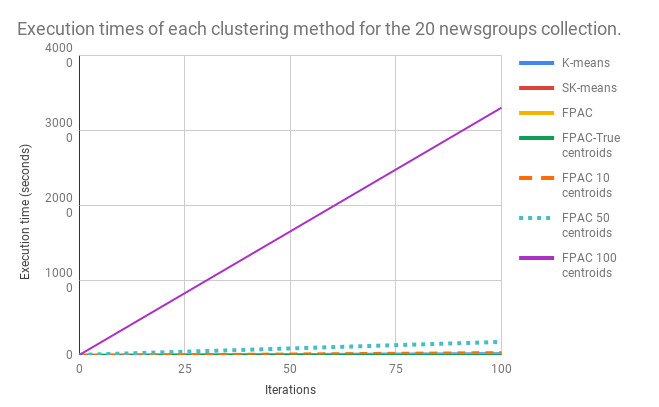
\includegraphics[scale=0.5]{graph20.png}
\end{figure}


\begin{figure}
\centering
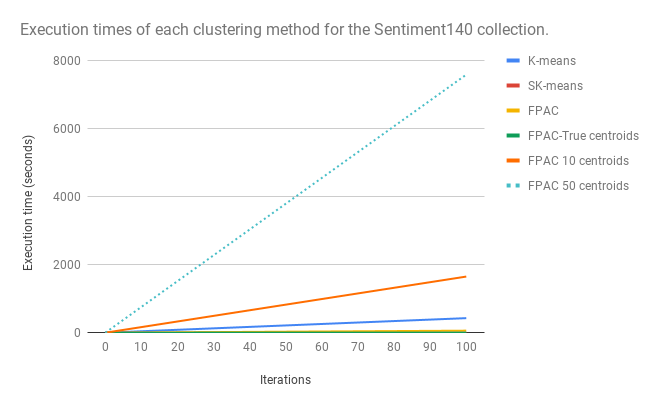
\includegraphics[scale=0.5]{graphtweets.png}
\end{figure}

\begin{table}[]
\centering
\caption{Comparasion betweet the clustering methods and their variants for the Sentiment140 dataset.}
\begin{tabular}{lllll}
\hline
Clustering algorithm & Purity  & NMI      & RI      & \begin{tabular}[c]{@{}l@{}}Change ratio\\ average\end{tabular} \\ \hline
K-means              & 0.50022 & 0.000014 & 0.49999 & 0.00414                                                      \\
SK-means             & 0.50135 & 0.000005 & 0.49999 & 0.49973                                                      \\
FPAC                 & 0.50022 & 0.000016 & 0.49999 & 0.50036                                                      \\
FPAC-True centroid   & 0.51440 & 0.000601 & 0.50040 & 0.46066                                                      \\
FPAC-10 centroids    & 0.50021 & 0.000000 & 0.49999 & 0.49997                                                      \\
FPAC-50 centroids    & 0.50189 & 0.000010 & 0.50000 & 0.49937                                                      \\ \hline
\end{tabular}
\end{table}


\begin{table}[]
\centering
\caption{Comparasion betweet the clustering methods and their variants for the 20 newsgruop dataset.}
\begin{tabular}{lllll}
\hline
Clustering algorithm & Purity  & NMI      & RI      & \begin{tabular}[c]{@{}l@{}}Change ratio\\ average\end{tabular} \\ \hline
K-means              & 0.12556 & 0.07351 & 0.70652 & 0.01005
 \\
SK-means             & 0.06800 & 0.00581 & 0.90464 & 0.94835                                                      \\
FPAC                 & 0.10962 & 0.02773 & 0.90221 & 0.95339 \\
FPAC-True centroid   & 0.17072 & 0.06257 & 0.90663 & 0.52449
 \\
FPAC-10 centroids    & 0.07004 & 0.00547 & 0.90464 & 0.93315 \\
FPAC-50 centroids    & 0.07084 & 0.00586 & 0.90464 & 0.86606 \\
FPAC-100 centroids    & 0.06818 & 0.00492 & 0.90462 & 0.78195 \\ \hline
\end{tabular}
\end{table}


\begin{itemize}
\item Por cada dataset una gráfica del NMI, Purity y RI
\item 
\end{itemize}
\section{Conclusions and future work}

%
% ---- Bibliography ----
%
% BibTeX users should specify bibliography style 'splncs04'.
% References will then be sorted and formatted in the correct style.
%
\bibliographystyle{splncs04}
\bibliography{references}
%
\end{document}
